\documentclass[a4paper]{article}

\usepackage{amsmath}
\usepackage{graphicx} % for eps files
\usepackage[hypcap]{caption} % link point to the top of the image
\usepackage{color}
\definecolor{links}{rgb}{0.21, 0.27, 0.45}
\usepackage[colorlinks=true,linkcolor=links]{hyperref}
% text corresponding to the target's type
\usepackage[nameinlink]{cleveref}

%% will prepend the section number to all equation numbers (amsmath)
\numberwithin{equation}{section}

%% Documentation to execute bash:
%%tex.stackexchange.com/questions/14186/how-can-i-provide-a-verbatim-unescaped-commandline-for-executing-with-write18
\def\exec{\begingroup\setexeccatcodes\innerexec}
\def\setexeccatcodes{\catcode`\#=12 \catcode`\%=12{}
	\catcode`\=12 \catcode`\$=12 \catcode`\^=12 \catcode`\\=12
}
\def\innerexec#1{\immediate\write18{\unexpanded{#1}}\endgroup}

\def\leer{\begingroup\setleercatcodes\innerleer}
\def\setleercatcodes{\endlinechar=-1}
\def\innerleer#1{\immediate\input{|#1}\endgroup}

% Function to get raw code and generate EPS
\newcommand\gnuplotcmd[2]{% arg 1: commands; arg 2: name of output file
	\exec{echo 'set terminal epslatex color colortext standalone;
		set output "#1.tex";
		#2;
		set output;' | gnuplot;}
	\exec{latex "#1.tex" &&
		dvips "#1.dvi" &&
		ps2eps -f -q "#1.ps" && mv "#1.eps" "../Figures/#1.eps";
		rm -f "#1".tex "#1".dvi ../Figures/"#1".tex;
	}
}

% Command to run gnuplot code and insert the result as picture (tight)
\newcommand\gnuplot[3]{ % First argument: caption. Second argument: name of file (and figure). Third
% argument: code
	% (all the commands are sent as a single line)
	\gnuplotcmd{#2}{#3}
	%% Make picture tight with epstool:
	%\exec{epstool --bbox --quiet --copy "#3".eps "#3".eps.mod}
	%\exec{mv "#3".eps.mod "../Figures/""#3".eps}
	\centering
	\includegraphics{../Figures/#2.eps}
	\caption{#1\label{fig:#2}}
}

% Command to run gnuplot code and insert the result as picture (tight)
\newcommand{\gnuplotfile}[3]{ % arg 1: caption; arg 2: name of eps file (and label);
% arg 3: file with gnuplot code

	% Add a line to replot and send to a file in gnuplot
	\exec{echo 'load "#3";
		set terminal epslatex color colortext standalone;
		set output "#2.tex";
		replot;
		set output;' | gnuplot}
	\exec{latex "#2.tex" &&
		dvips "#2.dvi" &&
		ps2eps -f -q "#2.ps" && mv "#2.eps" "../Figures/#2.eps";
		rm -f #2.tex #2.dvi;
	}
	% Add picture with caption and label
	\centering
	\includegraphics{../Figures/#2.eps}
	\caption{#1\label{fig:#3}}
}

% Command to execute maxima code and print it as LaTeX
\newcommand\maxima[1]{ %%$ \displaystyle\maxima{diff(f(x),x)} $
	%% Documentation
	%% tex.stackexchange.com/ questions/ 87095/ is-it-possible-to-write-all-mathematical-formulas-in-a-separate-file- and-add-the
	\exec{
		maxima --very-quiet -r ' % read and remove headings from maxima
		display2d: false'\$' % no fancy notation
		tex(#1)'\$ |  % convert to tex in maxima
		tr -d \$ | % remove dollar signs
		sed '/^'\$'/{d}' > /tmp/maxima.aux % dump output to file
	}
	\input{/tmp/maxima.aux} % read file
}

\begin{document}
% Create a dedicated folder for the Figures
\exec{[ ! -d ../Figures ] && mkdir ../Figures}

% Normal LaTeX equation (it will look nice, but not always make sense)
\begin{equation} \label{eq:GeneralVolumeIntegral}
	V=\int {\int {f\left(x , y , z\right)}{\;z}}{\;dA\left(x , y
	\right)}
\end{equation}


% example to use maxima notation:
\begin{subequations} \label{ChgEllipCoord}
	\begin{align}
		\maxima{r^2 = (x/a)^2 + (y/b)^2} \\
		\maxima{x = a*r*cos(\theta)} \label{ChgEllipCoord1}\\
		\maxima{y = b*r*sin(\theta)} \label{ChgEllipCoord2}
	\end{align}
\end{subequations}

This is a derivative with maxima code: $\displaystyle \maxima{diff(f(x),x))}$

% Example gnuplot code (finish every line with semicolon):
\begin{figure}[htb!]
	\gnuplot{Caption}{test}{
		set xlabel "$x$";
		splot tan(x), sin(x);
	}
\end{figure}
The figure depicted in \Cref{fig:test} is made with Gnuplot


%% Uncomment and change path to code to test loading from file:
%\begin{figure}[htb!]
%	\gnuplotfile{Caption
%	}{EllipticalFrustum}{path/file.gp}
%\end{figure}

\begin{figure}[htb!]
	\centering
	\gnuplotcmd{FileGnuplot}{
		% Example from the documentation demo_4.4/contours.1.gnu
		set samples 20, 20;
		set isosamples 21, 21;
		set contour base;
		set title "3D gnuplot demo - contour plot";
		set xlabel "X axis";
		set ylabel "Y axis";
		set zlabel "Z axis";
		set zlabel  offset character 1, 0, 0 font "" textcolor lt -1 norotate;
		splot x*y;
	}
	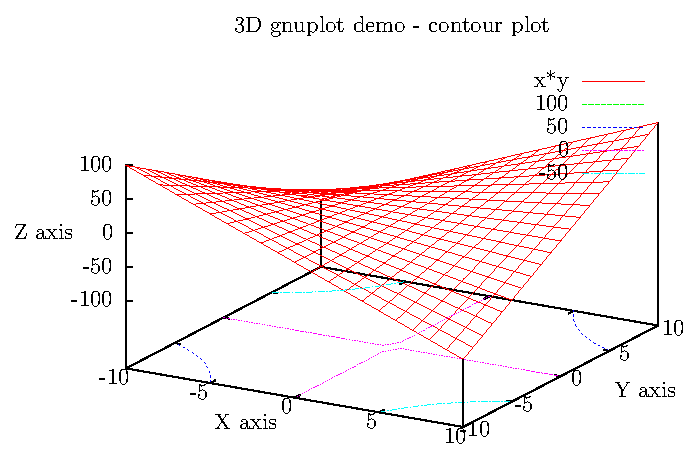
\includegraphics[]{../Figures/FileGnuplot.eps}
	\caption{My Caption \label{label}}
\end{figure}

\end{document}
